\section{Methods}

We manually designed strategies that organisms could use to cooperate in order to experimentally demonstrate that the DISHTINY platform selects for detectable hierarchical transitions in individuality.


\subsection{DISHTINY}

\begin{figure*}[t]
\begin{center}
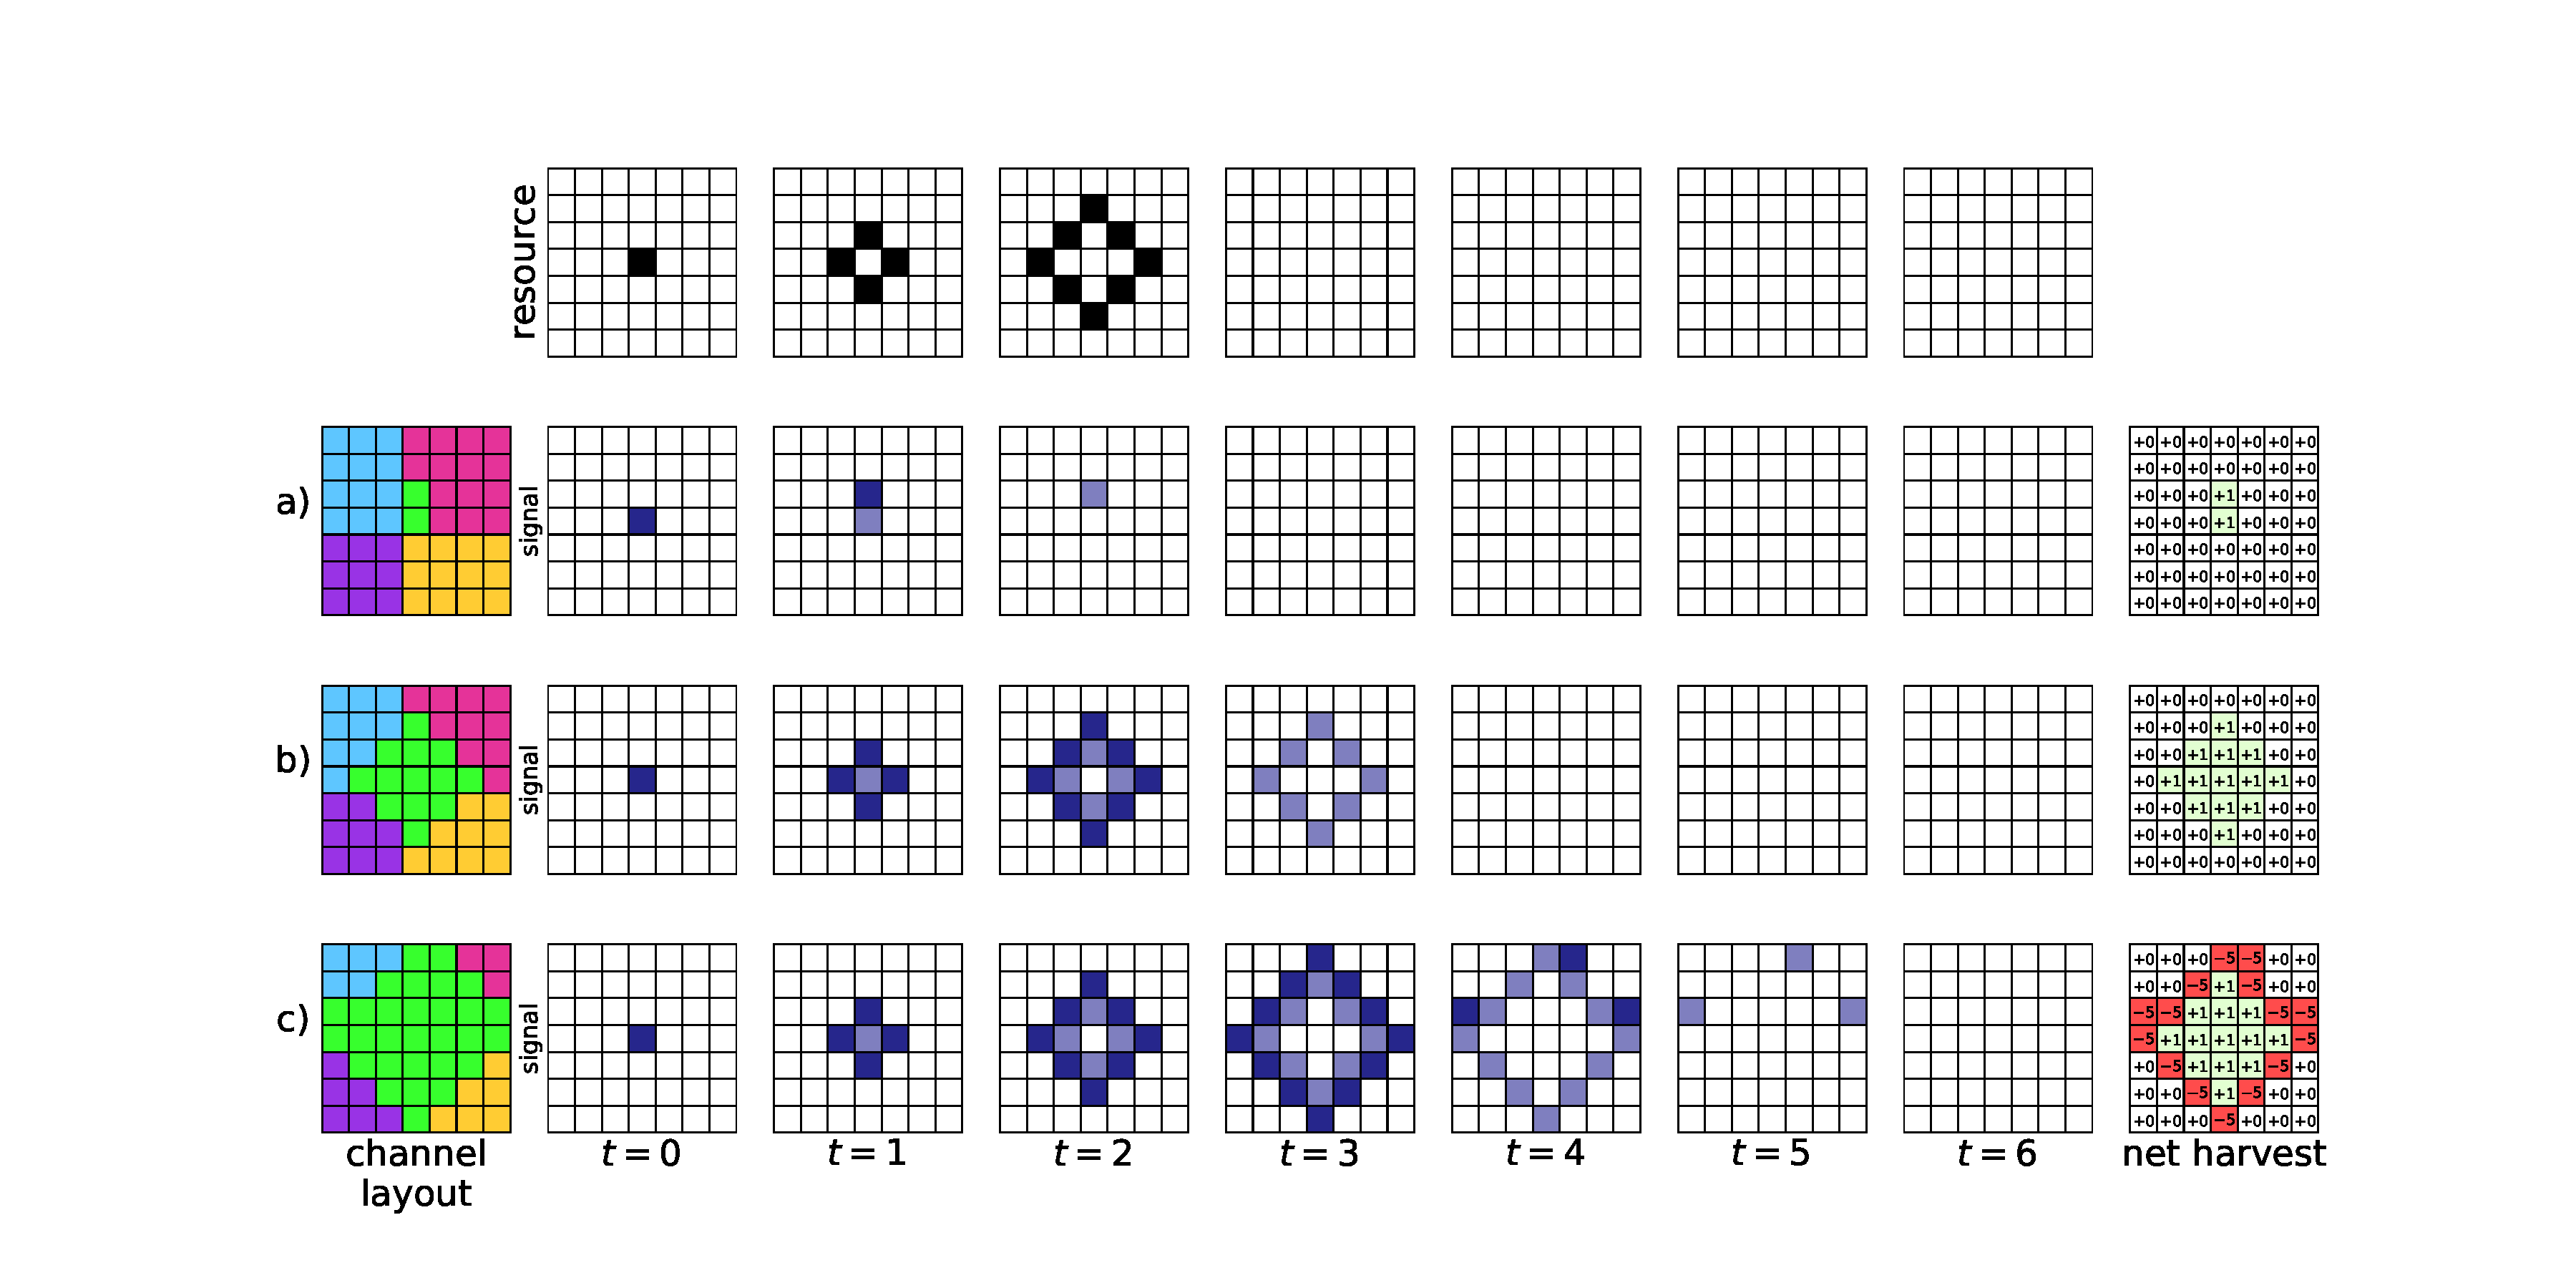
\includegraphics[width=2.0\columnwidth]{img/explanatory}
\caption{
\textbf{Activation signaling, and net resource collection for three different channel configurations during a resource wave event.}
At the top, a resource wave is depicted propagating over three updates and then ceasing for four updates (left to right).
In row $a$, a small channel-signaling group (far left, in green) is activated; tracking the resource wave (top) yields a small net resource harvest (far right).
In row $b$, an intermediate-sized channel-signaling group yields a high net resource harvest.
Finally, in row $c$, a large channel-signaling group incurs a net negative resource harvest.
In rows $a$, $b$, and $c$, dark purple indicates the active state, light purple indicates the quiescent state, and white indicates the ready state.
}
\label{fig:explanatory}
\end{center}
\end{figure*}


%We will begin by discussing the implementation of our artificial environment at a single hierarchical level, then lay out how the system scales to multiple levels.

% @CAO: We need to start by saying something about what these organisms are.  As of now the reader doesn't know if they are programs, neural networks, or what.  Technically these principles should work with any kind of organism, but I think the reader will be more comfortable having some information here.
Low-level organisms in DISHTINY consist of a set of values defining behavioral strategies, as well as one or more communication-channels where they can share information.  Over time, organisms also collect
a single continuous-valued resource and when they accrue enough, they may choose to pay $8$ units to reproduce.
%As shown Figure \ref{fig:explanatory},
Resources appear in waves that emanate from a single point.
With each simulation update, the resource wave advances one grid tile outward, disappearing when it reaches a predefined limit.
%The resource wave then ceases.
% @CAO This next sentence used way too many big words!
%Coincident with the inception of each resource wave,
Only the organism at the starting position of a resource wave is automatically notified about it, however they will send a signal to neighboring organisms sharing the same communications channel, which will continue to be propagated along that channel in a signal wave.  Only organisms notified of the resource can benefit from it;
%an activation-quiescence signal wave is triggered at the wave's center point.
%With every update, the signal wave passes to adjoining cells registered to the same channel as the cell it emanates from.
%The signal wave is not propagated to any cells on any other channel.
organisms not on the same channel (or without a continuous chain of signals) will ot be able to access the resource wave.
%In this way, cells sharing the channel of the cell where the resource wave originated are activated coincident with the resource wave.
%Example signal waves are shown in Figure \ref{fig:explanatory}.
%
%In order to obtain resource, a cell must be activated by a signal wave as the resource wave passes over.
%The cell at the center of a resource wave will always be activated and absorb resource.
%However, immediately adjacent cells can only obtain resource by the action of the signal wave --- by sharing the channel of the originating cell.
%Cells further off depend on a continuous path of cells extending from the originating cell that signal on the originating channel in order to obtain resource.
As shown in Example $a$ of Figure \ref{fig:explanatory}, the rate of resource collection is determined by the size of a channel signaling network; small or fragmented channel networks will tend to frequently miss out on resource as it passes over.

Technically, an activation cost is paid by each cell that is activated by a signal wave.
This cost is normally outweighed by the resource collected such that cells that activate in concert with a resource wave always take away a net benefit.
Recall, though, that resource waves have a limited extent.
Cells that activate outside of a resource wave or activate out of sync with the wave (due to an indirect path from the cell that originated the signal) pay a cost.
Cells that frequently activate erroneously use up their resource and die.
In our implementation, organisms that accrue a resource debt of $-11$ or greater are killed.
This scenario is depicted in Figure \ref{fig:explanatory}c.

In this manner, ``Goldilocks'' --- not to small and not too big --- same-channel signaling networks are selected for.
In our implementation, resource waves are seeded at a single location drawn  with uniform probability from the toroidal grid.
Based on this location, resource wave seeds are tiled over the toroidal grid
%so as to have kissing --- but non-overlapping --- extents.
such that their limits touch, but do not overlap.
All waves start and are updated synchronously; when they complete,
%Then, another
the next batch of resource waves is seeded.
This process ensures that selection for ``Goldilocks'' same-channel signaling networks is uniformly distributed over the toroidal grid.

Organisms may control the size and shape of their same-channel signaling group by strategic control of reproduction.
Three choices are afforded: whether to reproduce at all, where among the four adjoining tiles of the toroidal grid to place their offspring, and whether the offspring should be registered to the parent's signaling channel or should instead be registered to a random channel ID (int the range 1 to $2^{22}$). %4194303).
No guarantees are made about the uniqueness of an offspring's channel ID, but chance duplications are rare. % with respect to the channel IDs of the parent or other neighboring cells.

Hierarchical levels are introduced into the system through multiple instantiations of this resource wave/channel-signaling wave scheme.
In our experiments, we worked with two resource wave/channel-signaling levels, identified here as level zero and level one.
%On level zero, resource waves extended a radius of four toroidal tiles, granted a resource value of $+6$, to an activated organisms and cost a signaling activation penalty of $-5$ for a net of $+1$ resource.  On level one, resource waves extended a radius of twelve toroidal tiles, granted a resource value of $+6$, and cost a signaling activation penalty of $-5$.
On level zero, resource waves extended a radius of four toroidal tiles, while on level one they extended a radius of twelve toroidal tiles.  On both levels, activated organisms netted $+1$ resource from a resource wave, but suffered an activation penalty of $-5$ if no resource was available.

% Thus, each organism was a member of cooperating signaling groups, each determined by a unique channel ID --- a zero level signaling network and a one level signaling network.
We categorized organisms into signalling groups based on their channel IDs.
Due to the different limits of resource waves on different levels, level zero selects for smaller signaling networks and level one selects for larger networks.
We enforced hierarchical nesting of these signaling networks during reproduction:
%When creating an offspring, we only allowed a cell to generate an offspring with (1) identical zero- and one-level channel IDs, (2) new zero-level ID and identical one-level channel ID, or (3) new zero- and one-level channel IDs.
offspring may inerit neither channel, just the level one channel, or both channels.  It can not inherit only the level zero channel, while having a different level one channel.
% @CAO Given the international audience, I would NOT use the U.S. as an example.
%The distribution of IDs across the zero and one level channels can be envisioned like U.S. counties and states.
%Each county (i.e. zero-level channel network) is a member of exactly one state (i.e. one-level channel network); no county spans two states.
The distribution of IDs across the level one and level zero channels can be envisioned as countries and territories.  Each country (i.e. level-one channel network) may have many territories (i.e. level-zero channel network); no territory spans more than one country.
Figure \ref{fig:outcome_grids} depicts hierarchically nested channel states at the end of three evolutionary runs.

Channel IDs enable straightforward detection of an evolutionary transition in individuality.
Common channel IDs indicate a close relationship typically due to a recent bottleneck.  %Making channel ID a strictly inherited attribute and enforcing hierarchical nesting of channel IDs ensures reproductive bottlenecking and meaningful reproductive lineages at the level of the same-channel signaling network.
To recognize an evolutionary transition in individuality, we therefore evaluate
\begin{enumerate}
\item Do individuals with the same channel ID choose to share resources (e.g. cooperate)?
\item Is there division of reproductive labor between members of the same channel %(i.e. between individuals enveloped in a same-channel signaling network and those on the periphery)?
(e.g., do individuals at the periphery of a network behave differently from those in the interior?)
\end{enumerate}
If these conditions are met among organisms sharing the same level zero channel, we can conclude that a first-level transition in individuality has occurred.
Likewise, if these conditions are met among organisms sharing the same level one channel, we can conclude that a second-level transition in individuality has occurred.

\subsection{Organisms}

%We performed our experiments using organisms comprised of a set of 15 floating-point parameters.
DISHTINY organisms are composed of 15 floating-point parameters,
each describing a specific strategy component.
On reproduction, mutation was applied to each parameter independently with probability $0.00005$.
%We will overview each strategy parameter below.

%Parameters $A_0$ and $A_1$ modulate same-channel reproductive competition.
%Parameter $A_0$ is the probability an organism would to decline to replace an adjoining organism sharing the same level zero channel ID with an offspring.
%Parameter $A_1$ is the probability an organism would to decline to replace an adjoining organism sharing the same level one channel ID with an offspring.
%@CAO: I am naming the parametes below -- make sure you agree with my name choices!
The altruism parameters ($A_0$ and $A_1$) control the probability that an organism declines to replace an adjoining organism that shares the same level-zero ($A_0$) or level-one ($A_0$) channel ID with their offspring.
Mutation is performed by a redraw from the uniform distribution $U(-0.5,1.5)$ clamped to the range $[0,1]$.

Resource pool usage is controlled by the $P_{c}$, $P_0$, and $P_1$ parameters.
The $P_{c}$ parameter controls the proportion of resource collected into and paid from an organism's individual resource stockpile, while the $P_0$ and $P_1$ parameters, respectively, control the proportion of resources going into and out of the resource pools shared by organisms with identical level zero and level one channel IDs.
These parameters are initialized by a draw from $U(0.0, 1.0)$ and mutated by addition of a normal value drawn from $N(0.0,0.2)$ with the result clamped to the range $[0,1]$.
The set $P_{c}, P_0, P_1$ is always normalized to sum to 1.

Channel resource pools are identical to an organism's individual stockpile, except that any deficit is distributed evenly among the individual organisms.
On every update, individuals can spend from their individual stockpile to reproduce
%Then, in ascending level order, resource pools were afforded the opportunity to spend resource to reproduce.
%Resource pools carry out reproduction using the cell closest to the centroid of that the pool's channel-ID members that fails to decline to reproduce (i.e. via action of $A_0$ and/or $A_1$).
%As long as sufficient resource remains in the resource pool, the process is repeated to carry out another reproduction.
or a channel pool, with priority given to organisms nearest to the centroid of that pool's members.
As such, pool-funded reproduction fills in a channel-network from the inside out and can result in diamond-shaped same-channel signaling networks.
(Distance is measured using the taxicab metric.)

Channel caps $C_0$ and $C_1$ limit the size of same-channel signaling networks.
%Intuitively, they are caps on how many cooperators each organism wants in its zero-level signaling network and one-level signaling network, respectively.
When an organism reproduces, it checks the size of its level zero signaling network against $C_0$ and the size of its level one signaling group against $C_1$.
If neither cap is met or exceeded, then the organism will produce an offspring sharing both of its channel IDs.
If only the $C_0$ cap is exceeded, then the organism will produce an offspring with new level-zero ID, identical level-one channel ID.
Finally, if the $C_1$ cap is exceeded, then the organism will produce an offspring with new IDs for both channels.
These parameters are initialized by a draw from $U(0.0, 48.0)$ and mutated by adding a value drawn from $N(0.0,24.0)$ with the result clamped to be non-negative.

The endowment arameters $E_{c}$, $E_0$, and $E_1$ control the amount of resource provided to offspring.
This endowment is paid as an additional cost by the cell stockpile (or same-channel resource pool) funding a reproduction.
The full amount of the endowment is divided between the offspring's stockpile, level zero same-channel resource pool, and level one same-channel resource pool according to the offspring's parameters $P_{c}$, $P_0$, and $P_1$.
Specifically, $E_{c}$ is the endowment amount paid to an offspring that shares the both channel ID of the parent;
$E_0$ is the endowment paid to an offspring that shares just the level one channel ID of the parent;
and $E_1$ is the endowment paid to an offspring that shares neither the level-zero nor level-one channel ID of the parent.
Endowed resources help new-channel propagules to rapidly grow their signaling network in order to begin collecting resource at a competitive rate to other well-established signaling networks.
These parameters are initialized by a draw from $U(0.0, 3.0)$ and are mutated by addition of a value drawn from $N(0.0,10.0)$ with the result clamped to be non-negative.

Parameters $M_{c}$, $M_0$, and $M_1$ control the attempt of suicide on genetic damage.
Each time that a mutation occurs during reproduction, the mutated offspring attempts suicide with probability $M_{c}$ if it shares both channel IDs of its parent, probability $M_0$ if it shares just the level one channel ID of its parent, and probability $M_1$ if it shares neither channel ID of the parent.
The $M_x$ value applied is from the offspring's genotype after mutation.
Attempted suicide succeeds %with a probability of $0.8$.
80\% of the time.
This capacity enables first- or second-level individuals to combat somatic mutation.
Initialization and mutation each of these parameters is performed by a redraw from the distribution $U(-0.5,1.5)$ clamped to the range $[0,1]$.

Finally, parameters $S_0$ and $S_1$ affect offspring placement.
If an organism is placing an offspring with identical channel IDs, the four possible sites for offspring placement are considered in order of increasing distance from the centroid of the parent's level zero signaling network.
If an organism is placing an offspring with identical level one channel ID, but different level zero channel ID, the four possible sites for offspring placement are considered in order of increasing distance from the centroid of the parent's level one same-channel signaling network.
Otherwise, the four possible sites for offspring placement are considered in a random order.
These parameters were included to enable more exacting control of
Initialization and mutation is performed by a draw from the distribution $U(-0.5,1.5)$ clamped to the range $[0,1]$.

\subsection{Experiments}

We performed experiments to assess the evolutionary trajectories of populations %of organisms
in the DISHTINY environment.
We seeded each tile on the $120 \times 120$ toroidal grid with a randomized organism and ran the simulation for 20 million updates.
We performed 33 replications of this experiment, each taking approximately 60 hours.
Across all successive 10,000 update segments of all replicates, the mean number of cellular generations elapsed per 10,000 updates was 11.3 with a standard deviation of 1.9 cellular generations per 10,000 updates.

We observed evolutionary outcomes that resembled zero-, first-, and second-level individuality.
To assess the relative fitness of these evolved organisms, we ran ecological competitions between three genotypes --- one selected as the most common genotype from the evolutionary run where the greatest mean $P_{c}$ was observed, one selected as the most common genotype from the evolutionary run where the greatest mean $P_0$ was observed, and the other selected as the most common genotype from the evolutionary run where the greatest mean $P_1$ was observed.
We seeded each ecological run with three copies of each genotype, uniformly spaced over the toroidal grid with random arrangement. We ran these competitions for 2 million updates with mutation disabled.
We performed 191 replications of this experiment, each taking approximately 6 hours.


\subsection{Implementation}


We implemented our experimental system using the Empirical library for scientific software development in C++, available at \url{https://github.com/devosoft/Empirical}.  The code used to perform and analyze our experiments, our figures, data from our experiments, and a live in-browser demo of our system is available via the Open Science Framework at \url{https://osf.io/ewvg8/}.
